\begin{enumerate}
	\item Exercício
	
	Esboçe a região de integração e o sólido cujo volume é dado pela integral abaixo:
	\begin{equation*}
		\int_0^1 \int_0^1 \left(4 - x - 2y\right)\, dx dy
	\end{equation*} 
		
	\begin{figure}[htb]
		\caption{Integrais duplas - Aula 9 - Exercício I}
		\label{v09_a09_e01}
		\centering
		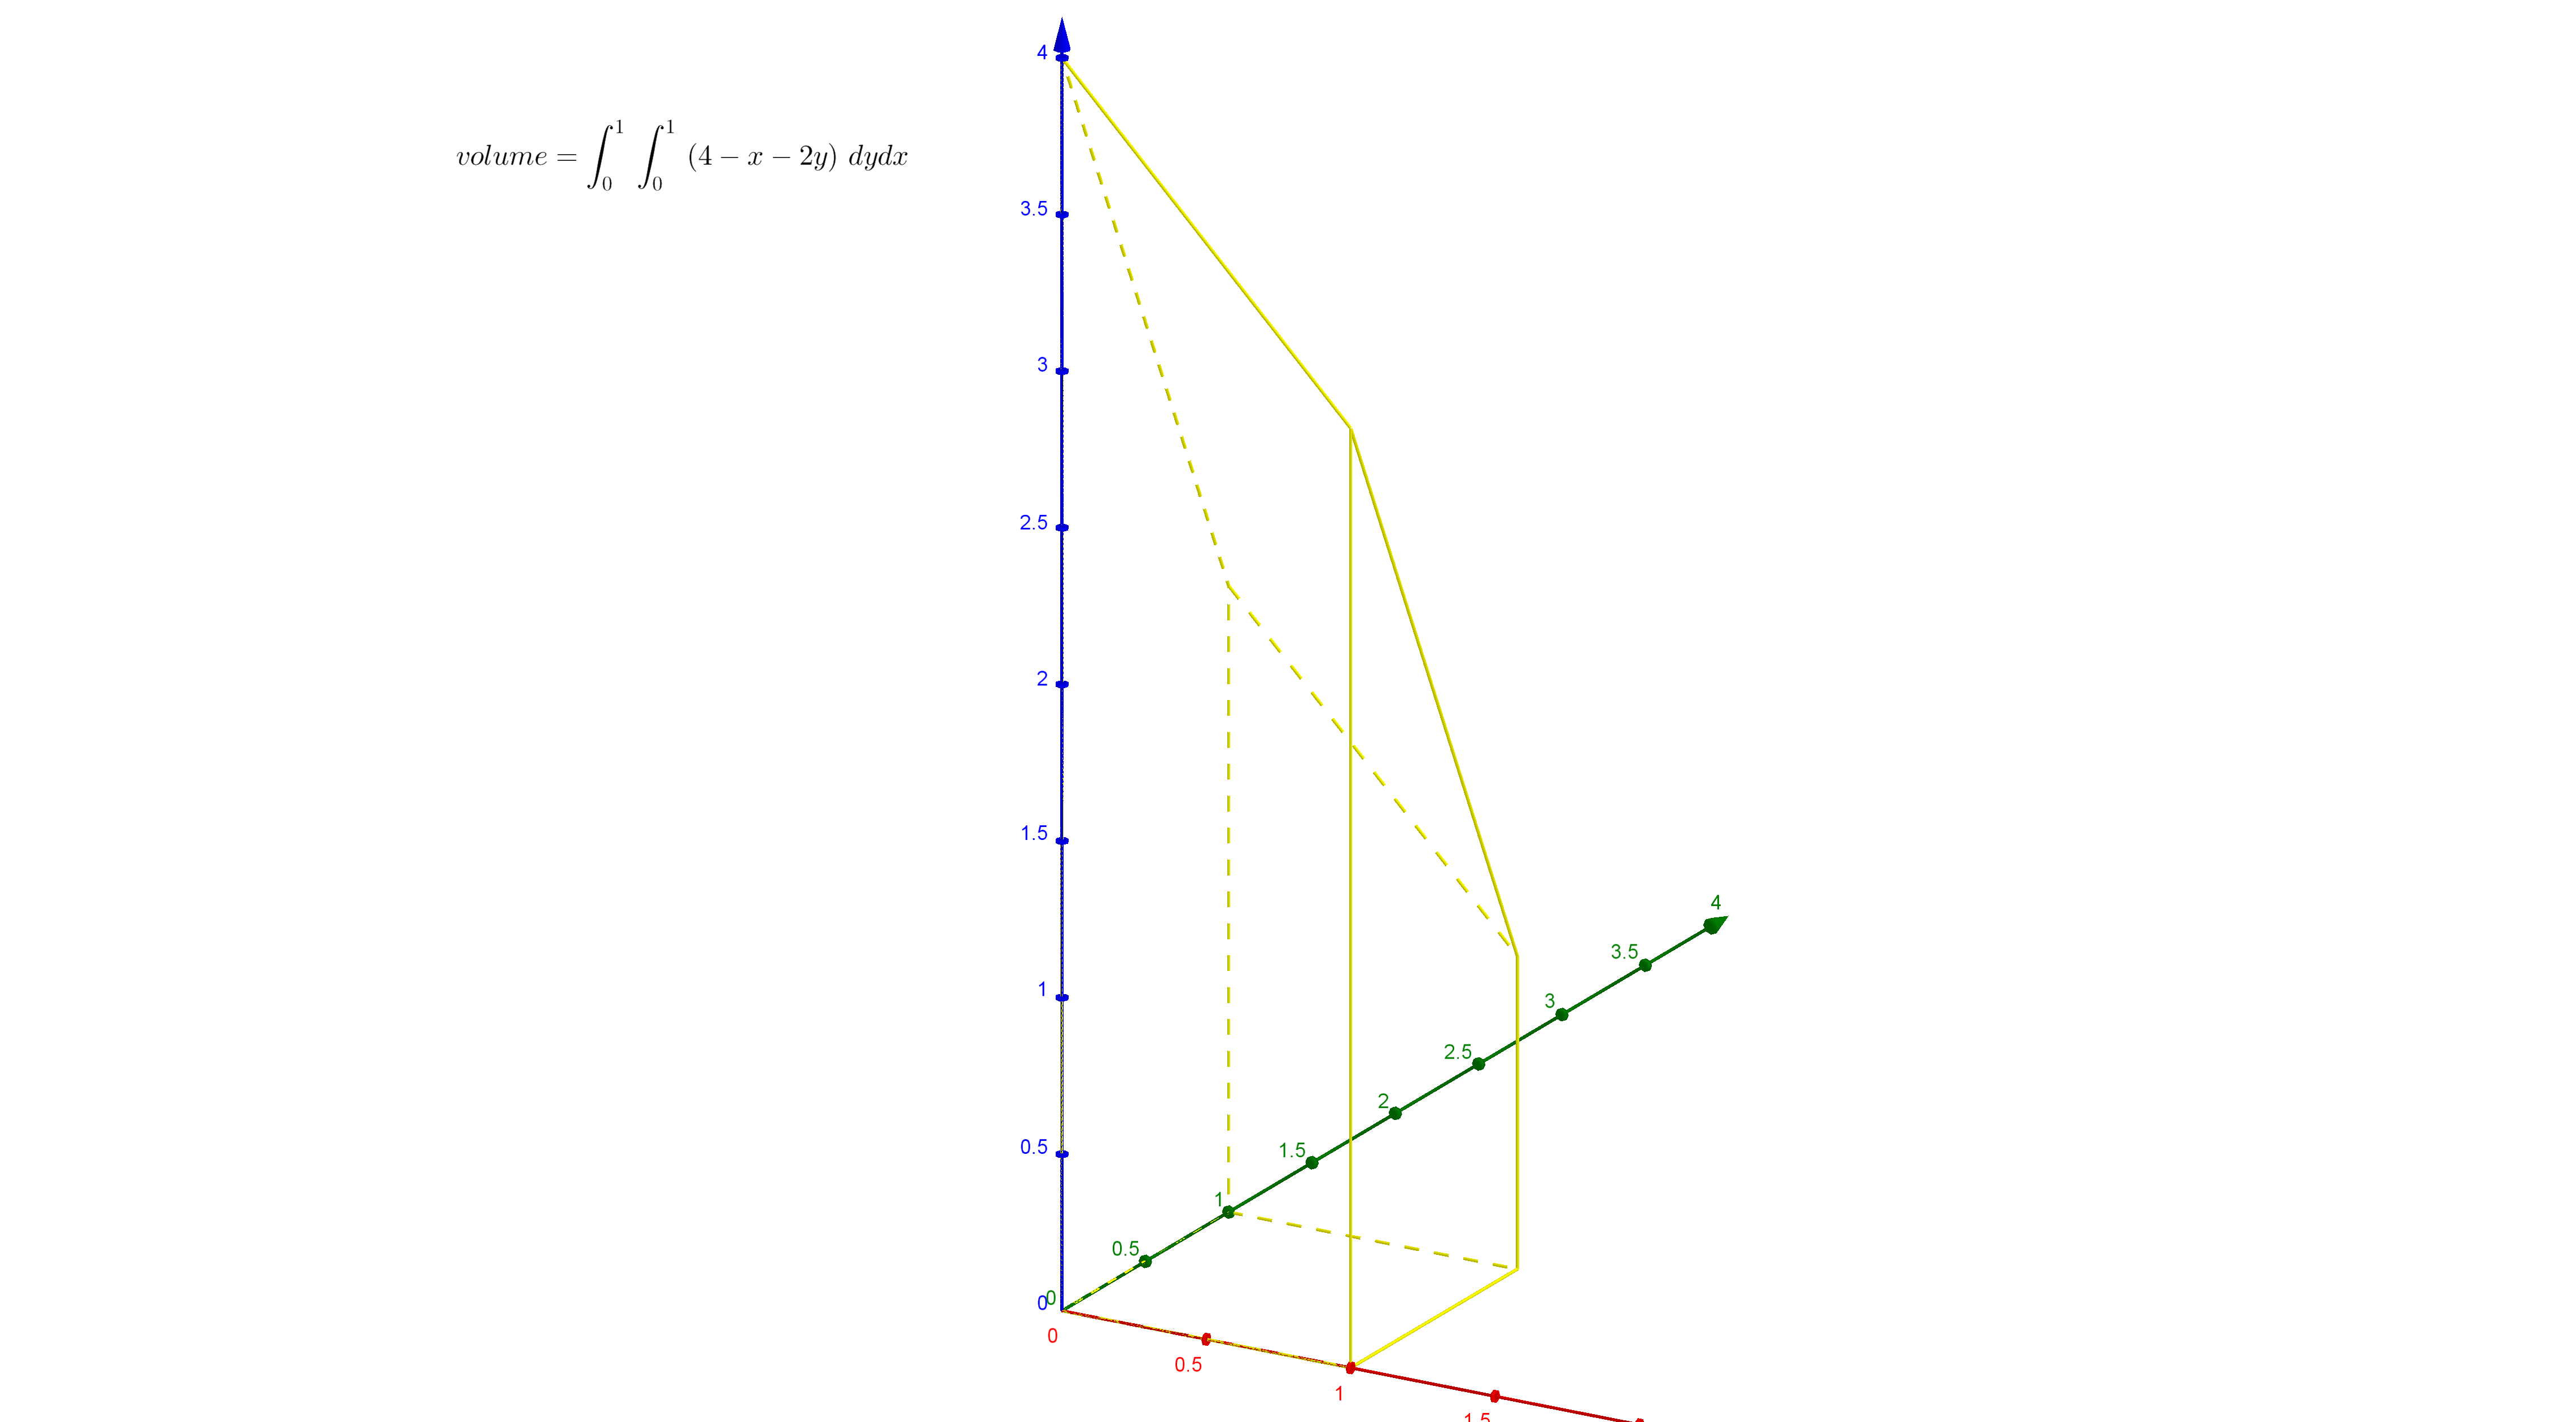
\includegraphics[width=0.5\textwidth]{v09_a09_e01.png}		
	\end{figure}
	
	\begin{gather*}
		v = \int_0^1 \int_0^1 \left(4 - x - 2y\right)\, dy dx = \int_0^1 dx \left(4\int_0^1 dy - x\int_0^1 dy - 2\int_0^1 y\, dy\right) =\\ 4\int_0^1 dx \int_0^1 dy - \int_0^1 x\, dx \int_0^1 dy - 2\int_0^1 dx \int_0^1 y\, dy =\\ 4[x]_0^1 [y]_0^1 - \left[\dfrac{x^2}{2}\right]_0^1 [y]_0^1 - 2[x]_0^1 \left[\dfrac{y^2}{2}\right]_0^1 = 4 - \dfrac{1}{2} - \overstrike{2}\dfrac{1}{\overstrike{2}} = \frac{8 - 1 - 2}{2} = \dfrac{5}{2} = 2,5	
	\end{gather*}	
\end{enumerate}